%%
%% paper04 — 独立小论文稿(中文)
%% 模板: ACM acmart manuscript。正文已与旧 NOSR/HMACSP 叙事脱钩,仅保留版式骨架。
%% 编译: XeLaTeX(必须;见下方 ctex 说明)。
%%
\documentclass[manuscript,screen,review]{acmart}

%% ===================== 中文支持 =====================
%% scheme=plain: 只接管中文字体与断行,不改写 acmart 的章节名。
%% fontset=windows: 本机宋体/黑体; Overleaf/Linux 可改为 fontset=fandol。
\usepackage[UTF8,scheme=plain,fontset=windows]{ctex}

\usepackage{algorithm}
\usepackage{algorithmicx}
\usepackage{algpseudocode}
\usepackage{pifont}
\usepackage{makecell}
\providecommand{\checkmark}{\ding{51}}
\newcommand{\cmark}{\ding{51}}
\newcommand{\xmark}{\ding{55}}
\newcommand{\omark}{\(\circ\)}
\usepackage{threeparttable}
\usepackage{tikz}
\usetikzlibrary{positioning,arrows.meta,calc,shapes,shadows}
\usepackage{xcolor}
\usepackage{amsmath}
\usepackage{bm}
\DeclareMathOperator*{\argmin}{arg\,min}
\DeclareMathOperator*{\argmax}{arg\,max}
\usepackage{multirow}
\usepackage{enumitem}
\usepackage{booktabs}
\usepackage{graphicx}
\setlength{\headheight}{20.48303pt}

%% 机制缩写:主语是闭包,不是「修复框架」
\providecommand{\STRC}{\textsc{STRC}}
\newcommand{\TBD}[1]{\textcolor{red}{\textbf{[待补:} #1\textbf{]}}}

\usepackage{amsthm}
\newtheorem{assumption}{假设}
\newtheorem{definition}{定义}
\newtheorem{problem}{问题}
\newtheorem{remark}{注}
\newtheorem{prop}{命题}
\newtheorem{lem}{引理}

\AtBeginDocument{%
  \providecommand\BibTeX{{%
    Bib\TeX}}}

\setcopyright{acmlicensed}
\copyrightyear{2026}
\acmYear{2026}
\acmDOI{XXXXXXX.XXXXXXX}

%%\acmSubmissionID{123-A56-BU3}

\begin{document}

%% =====================================================================
%% 标题:独立小论文用「任务图覆盖不到」钩子;大论文章题另用「闭包上的有界修复」
%% =====================================================================
\title[任务图覆盖不到的级联损坏]{任务图覆盖不到的级联损坏:无冲突柔性作业车间中的时空预约闭包}

\author{Qi Yu}
\email{230240012@seu.edu.cn}
\orcid{0009-0008-7843-6345}
\affiliation{%
	\department{School of Cyber Science and Engineering}
	\department{Key Laboratory of Computer Network and Information Integration}
	\institution{Southeast University}
	\city{Nanjing}
	\state{Jiangsu}
	\country{PR China}
}

\author{Wei Li}
\orcid{0009-0001-0949-329X}
\email{xchlw@seu.edu.cn}
\authornote{corresponding author}
\affiliation{%
	\department{School of Computer Science and Engineering}
	\department{Key Laboratory of Computer Network and Information Integration}
	\institution{Southeast University}
	\city{Nanjing}
	\state{Jiangsu}
	\country{PR China}
}

\renewcommand{\shortauthors}{Yu and Li}

%% =====================================================================
%% 摘要
%% 骨架:背景缺口 → 主张(边界在预约图) → 对象 STRC → 用法(有界修复) →
%%       与全局重解互补 → 实验钩子(不把创新挂在「又一个修复算法」上)
%% =====================================================================
\begin{abstract}
当柔性作业车间的运输被建模为常数时间矩阵时,车辆互不阻挡,延误只是布局属性;
一旦 AGV 在显式走廊网络上以时间窗预约通行,延误成为一车施加给另一车的量,
排程的可行性便同时写在任务依赖与预约表上。现有局部重调度多在\emph{任务依赖图}
上划影响域:由故障工序或故障智能体作种子,再按工序/指派邻域扩张。
这一做法覆盖一类扰动(机器故障、插单等),却系统性地漏掉另一类——
走廊阻断、路段降速等\emph{并不改动任何工序指派}的扰动。
对后者,任务图上直接受扰集合为空,框架会判「无需重调度」,而预约表上已有大片占用失效,
并沿「谁挡了谁」向外级联。本文把这一缺口表述为:\textbf{任务图覆盖不到的级联损坏}
——不是检测漏检,而是任务图这一表示本身不含预约级联通道。

本文主张:在无冲突路由设定下,扰动的影响边界必须定义在\emph{时空预约图}上。
我们提出时空预约影响闭包(\STRC, Spatiotemporal Reservation Closure):
以与扰动时窗重叠的预约为种子,沿等待阻塞、同车接续、同工件接续与机器链等依赖取传递闭包,
得到可释放、可冻结的损坏范围。闭包是对象;在闭包上做有界修复(改路,失败则扩大释放域)
是把该对象用起来的手段,而非本文的主语。
在同一无冲突执行器与同挂钟协议下,我们对照任务图影响域、以及热启动全局重解:
走廊类扰动上任务图种子为空而 \STRC{} 非空且原排程不可行;同修复引擎下仅换边界定义时,
任务图边界无法恢复可行而闭包边界可以;闭包路径以毫秒级恢复可行,
相对热启动全局重解改动的预约更少、耗时低两至三个数量级,而后者在更宽预算下
取得更优完工时间——二者互补而非互相替代。

实验在争用型算例族上复现上述对照:走廊阻断上任务图影响域为空而闭包非空;
同引擎下仅换边界即可决定能否恢复可行;扰动比例扫描下闭包路径以毫秒级达到
全样本可行,热启动重解以秒级预算取得更优完工时间。
本文不宣称在完工时间上全面优于全局搜索;贡献在于指出并修正影响边界的划定对象,
并给出与显式预约表设定相匹配的局部恢复路径。
\end{abstract}

\keywords{柔性作业车间调度, AGV 无冲突路由, 时空预约表, 影响闭包,
级联损坏, 局部重调度, 走廊阻断}

%% CCS 投 ACM 时用官方工具重生成;非 ACM 可删。
% \begin{CCSXML}
% <ccs2012>...</ccs2012>
% \end{CCSXML}
% \ccsdesc[500]{Theory of computation~Scheduling algorithms}
% \ccsdesc[300]{Applied computing~Industry and manufacturing}
% \ccsdesc[300]{Computing methodologies~Planning and scheduling}

\maketitle

%% =====================================================================
\section{引言}
\label{sec:introduction}
%% =====================================================================

\subsection{背景与动机}

考虑运输的柔性作业车间调度长期依赖一个便利假设:工件在机器之间的移动时间是一张
按位置索引的常数矩阵。该假设等价于默认车辆互不干扰——行驶时间是布局的固有属性,
而不是路由决策的结果。一旦有限车队共享稀疏走廊网络,并以半开时间窗预约走廊资源,
上述默认便不再成立:一辆车的让行会推迟另一辆车的到达,进而推迟工序开工与后续预约。
此时,一份「可行排程」同时包含工序指派、排序与一张走廊预约表;扰动不仅可以打坏任务,
也可以只打坏预约。

静态一体化排程的研究已经表明,显式无冲突路由与柔性指派的耦合会改变指派优劣次序,
而把拥堵写进评价、在决策中查询冲突信息,是构建高质量排程的关键路径~\cite{vanos2026exact,li2026framework,sun2023integrated}。
那些工作主要回答:\emph{如何在信息完备时建出一份好的无冲突排程}。
车间运行中的问题不同:在执行时刻 \(t_{\mathrm{now}}\) 发生扰动之后,
\emph{损坏落在何处、改到何处才够}——以及这件事能否在毫秒至百毫秒量级完成,
而不必每次都重新打开种群搜索。

\subsection{任务图覆盖不到的缺口}

局部重调度文献常用任务依赖图界定影响域:由直接失效的工序或智能体作种子,
再按工件后继、机器链或固定跳数 \(\theta\) 扩张,然后只对影响域内任务重优化。
这一边界在「扰动本身就是一个任务事件」时往往合理——例如机器故障使若干工序无法按原指派执行。
然而在显式预约模型里,存在一类扰动,其作用对象是走廊时窗而非工序指派。
典型例子是走廊阻断:某走廊在 \([t_a,t_b)\) 不可通行。
阻断不修改任何机器指派或工序顺序,因此任务图上的直接受扰集合
\(T_{\mathrm{direct}}=\varnothing\);若框架以「空影响域」推出「无需重调度」,
则会系统性漏报——原排程中落在该时窗的预约已经失效,并可能通过等待阻塞关系
迫使后续车辆改道或推迟,形成\emph{预约表上的级联}。

本文强调用语:所谓「覆盖不到」,指的是任务图这一\emph{表示}天然不含预约级联通道,
而不是传感器漏检或算法偶然漏报。在常数运输矩阵模型里,这类损坏甚至无法被写下——
走廊不是资源,预约表不存在。因此,问题本身附着于无冲突路由与显式预约设定;
这不是应用上的窄化,而是表述该缺口所必需的模型前提。

据此,我们区分两类扰动(后文形式化):
\begin{itemize}[leftmargin=1.5em,itemsep=0.25em]
\item \textbf{A 类}(触碰任务图):机器/机械臂故障、加工时间显著偏差、插单等——
任务图种子通常非空;此时任务图边界与预约闭包可能接近,但不是本文主检验对象。
\item \textbf{B 类}(主要触碰预约表):走廊阻断或降速、局部通行权临时取消等——
任务图种子可为空,预约表种子与闭包非空。
\end{itemize}
B 类构成问题层的一击反例:不是「需要更好的修复启发式」,而是
「局部重调度文献在无冲突设定下一直可能划错影响边界」。
图~\ref{fig:motivate} 对照这一缺口:左侧任务图种子为空因而判「无需重调度」;
右侧预约表上阻断窗命中种子并沿让行/接续边形成闭包。

\begin{figure}[t]
\centering
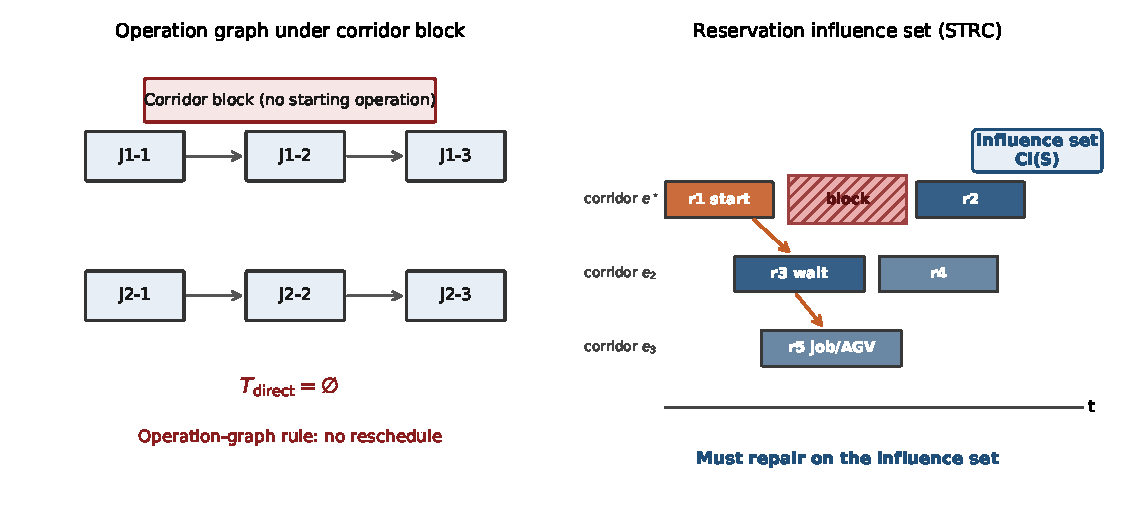
\includegraphics[width=\linewidth]{figures/fig_strc_motivate}
\caption{动机示意。左:走廊阻断不命中任何工序/机器,任务图直接集为空。
右:同一扰动在预约表上产生种子,并沿阻塞与接续关系级联为时空预约闭包。}
\label{fig:motivate}
\end{figure}

\subsection{主张与方法预告}

本文主张三句话。第一,在无冲突柔性作业车间中,扰动影响边界应定义在时空预约图上,
而非仅定义在任务依赖图上。第二,正确的影响对象是\emph{时空预约影响闭包}
(\STRC):以失效预约为种子,沿预约阻塞与调度接续关系取传递闭包;
闭包之外的预约在结构上与种子无依赖,从而「局部」第一次对应一个可检验的对象,
而不是启发式剪枝半径。第三,闭包上的有界修复——释放闭包内预约、外侧冻结、
原车改路,失败则沿工件/车辆链扩大释放——是闭包的应用;升级阶梯中更贵的协调
(换车、改派、改序)可以随后展开,但不是本文创新的挂靠点。

与「每次扰动都热启动全局重解」相比,\STRC{} 路径回答的是另一侧问题:
在紧响应预算下能否快速恢复可行,并在结构上把修改限制在闭包内。
外侧预约字段的逐条不变是给定边集与预提交成功时的充分条件
(命题~\ref{prop:outside}),而非实验上恒成立的口号;相对全局重解,
闭包路径通常改动更少、响应更快。
实验将表明二者互补——闭包修复以极短耗时恢复可行;全局重解在固定挂钟预算下
常取得更优完工时间——因而正确叙事不是「取代搜索」,而是「测量损坏范围,
再决定用多便宜的协调就够」。

\subsection{贡献}
\label{sec:contributions}

按问题层、框架层、机制层、方法层组织,本文贡献如下。

\begin{enumerate}[leftmargin=1.6em,itemsep=0.4em]
\item \textbf{问题层:指认任务图覆盖不到的级联损坏。}
在显式走廊预约下形式化 B 类扰动:按任务图直接集的常规定义,
走廊阻断给出 \(T_{\mathrm{direct}}=\varnothing\);同时证明当预约种子非空时
原排程仍不可行,从而「空影响域 \(\Rightarrow\) 无需重调度」失效。
该缺口在常数运输时间模型中不可表述。

\item \textbf{框架层:先测量、再有界协调。}
将动态恢复组织为「闭包划定释放集 \(\rightarrow\) 外侧冻结 \(\rightarrow\)
闭包内最低必要协调」,与「打开种群搜索做全局重解」对照而不混为一谈。
测量优先于协调;修复是框架的第二步而非标题主语。

\item \textbf{机制层:时空预约影响闭包(\STRC)。}
定义种子、依赖边与传递闭包;证明结构闭合性
(闭包外不是闭包内顶点的出边后继),并给出外侧字段不变的\emph{充分条件}
(预提交成功且不扩域时)。同引擎消融表明:贡献主要来自边界定义
(任务图域 vs 闭包),而非某次改路启发式的细节。

\item \textbf{方法层:闭包上的有界恢复与对照协议。}
实现第 1 级改路及失败扩域再修;在统一无冲突执行器与同挂钟协议下,
对照任务图边界臂与热启动全局重解臂,报告可行性、耗时、预约变动与完工时间,
并给出扰动规模 \(\varphi\) 扫描下的互补关系。
\end{enumerate}

\subsection{与静态一体化排程工作的关系}
\label{sec:relation_static}

本文可独立阅读。若读者熟悉同一场景下的静态闭环双层排程工作,则二者关系可一句话概括:
\textbf{同一车间、同一预约表;前者用预约表构建排程,本文用预约表定位损坏。}
共享对象是显式路网、走廊独占与半开时窗预约;区别在时机与算法形态——
静态工作在 \(t=0\) 做种群搜索以最小化完工时间,本文在 \(t_{\mathrm{now}}\)
做单解有界恢复以恢复可行并把修改锚定在预约闭包上。
阻塞关系在前者可用于派车或诊断,在本文用于构造影响闭包。
独立阅读时,上述静态工作视为相关文献即可。

\subsection{篇章结构}

第~\ref{sec:related_work}~节回顾局部重调度、无冲突路由一体化调度与影响域方法。
第~\ref{sec:problem}~节给出系统模型、扰动二分与恢复问题陈述。
第~\ref{sec:strc}~节定义 \STRC{} 并陈述包含性(图~\ref{fig:closure})。
第~\ref{sec:repair}~节描述闭包上的有界修复与扩域策略(图~\ref{fig:framework})。
第~\ref{sec:experiments}~节报告实验,并以案例甘特衔接统计与时间轴。
第~\ref{sec:conclusion}~节总结并讨论局限。

%% =====================================================================
\section{相关工作}
\label{sec:related_work}
%% =====================================================================

本文将三条线索并置:动态局部重调度如何划影响域、带运输的柔性作业车间如何建模行驶时间,
以及无冲突路由下静态一体化排程已走到何处。缺口出现在三者的交界——显式预约已经存在,
而动态方法仍主要在任务图上划界。

\subsection{动态重调度与任务图影响域}

作业车间动态重调度的经典综述区分完全重调度与修复式/局部重调度,
并强调稳定性与响应时间~\cite{vieira2003rescheduling,ouelhadj2009survey}。
反应式规则与右移类方法响应快但缺少对「改哪些任务才够」的显式边界~\cite{dalcastagne2020reactive};
滚动时域与分解式方法试图在规模与质量之间折中~\cite{zeitrag2025novel,zhao2019decomposition}。
当扰动被建模为机器故障、工序延误或插单时,以故障智能体或失效工序为种子、
在任务依赖图上按深度或邻域扩张影响域,是自然且常见的做法。
这类边界对 \emph{A 类}扰动通常可用:种子落在任务图上,扩张沿着工件后继与机器链进行。
其隐含前提是——扰动首先是一个任务事件。一旦扰动只使走廊时窗失效而不改指派,
该前提不再成立,任务图种子可以为空,而排程已不可行。

\subsection{常数运输时间下的 FJSP--AGV}

考虑运输车辆的柔性作业车间调度已有系统综述~\cite{xin2025review}。
近期组合优化工作仍普遍把行驶时间取为按位置索引的常数矩阵,
并在此之上发展约束规划、元启发式与知识引导搜索~\cite{meng2025cp,qin2026knowledge,fu2025integrated}。
在该建模约定下,车辆互不占用同一时空资源,延误不是一车施加给另一车的量;
走廊阻断这类事件甚至没有对应的模型对象。因此,「任务图覆盖不到的预约级联」
在常数矩阵文献中既不会被提出,也无法被检验——这不是那些工作的缺陷,
而是本文问题附着于另一建模层级的原因。

\subsection{无冲突路由与静态一体化}

无冲突多机器人路径规划把走廊/边的时空占用作为一等约束,
但任务集合及其端点常由外部规划器给定~\cite{zhang2024guidance};
制造场景中的拥堵感知派车亦常以局部密度等代理量驱动选车,
而不回头改机器指派~\cite{kim2026congestion}。
把柔性指派与无冲突运输耦合的工作相对较少。
van Os 与 Basten~\cite{vanos2026exact} 形式化了带无冲突运输约束的柔性作业车间调度问题,
并以分解方法给出可证最优基准;两阶段方案先固定排产再消解车辆冲突~\cite{sun2023integrated};
亦有以学习层排产、路径层消冲突并以有限反馈连接的框架~\cite{li2026framework}。
这些工作主要回答静态或准静态下如何\emph{构建}可行且高质量的一体化排程。
它们留下的动态问题是:当执行中出现扰动时,损坏是否仍应只在任务图上测量?
若下层已维护走廊预约表,影响边界能否、以及应当否改写到预约图上?

\subsection{本文定位}

相对局部重调度文献,本文不提出新的通用分段框架,而指认无冲突设定下
任务图边界对 B 类扰动的系统性失效,并把正确对象定义为时空预约影响闭包。
相对静态一体化文献,本文复用同一类显式路网与预约执行器,但把算法形态从种群搜索
换为单解有界恢复,主指标从完工时间增益转为漏报与否、可行性、耗时与预约稳定性。
与「扰动后热启动全局重解」的关系是互补对照,而非声称在完工时间上全面更优。

%% =====================================================================
\section{问题描述}
\label{sec:problem}
%% =====================================================================

\subsection{系统设定与记号}
\label{sec:system_brief}

我们采用带无冲突运输约束的柔性作业车间设定~\cite{vanos2026exact} 的执行期版本,
记号与静态闭环解码器对齐,此处只保留后文需要的对象。

车间路由图 \(G=(V,E)\) 强连通;每条走廊 \(e\in E\) 为排他资源,通行时间 \(\tau_e\) 已知。
占用记为半开区间。\(n\) 个工件、机器集合 \(M\)、车队 \(K=\{1,\ldots,N_A\}\)。
工序 \(O_{ji}\) 的候选机器集为 \(\Omega_{ji}\subseteq M\)。
一份完整排程
\[
\mathcal{S}=(x,\,\pi,\,y,\,R)
\]
包含机器指派 \(x\)、工序扫描序 \(\pi\)、车辆指派 \(y\),以及预约表
\[
R=\bigl\{\,r=(e,\,[t^s,t^e),\,k,\,u)\,\bigr\},
\]
其中 \(k\in K\) 为车辆,\(u\) 为任务标签(空载/满载段)。
路径只占用 \(R\) 报告为空闲的时窗,从而构造性保持无冲突。

任务依赖图 \(G_T=(T_T,E_T)\) 以工序(或工序级任务 id)为顶点,
边为工件前后约束;它\emph{不}包含走廊占用之间的阻塞边。
预约依赖图 \(G_R=(R,E_R)\) 的顶点为 \(R\) 中的预约记录,边集见第~\ref{sec:strc}~节。

\begin{table}[t]
\centering
\caption{本文常用记号}
\label{tab:notation}
\small
\begin{tabular}{@{}ll@{}}
\toprule
\textbf{符号} & \textbf{含义} \\
\midrule
\(G=(V,E)\) & 走廊路网 \\
\(R\) & 走廊预约表(半开占用区间集合) \\
\(G_T\) / \(G_R\) & 任务依赖图 / 预约依赖图 \\
\(\mathcal{S}^0,\mathcal{S}'\) & 扰动前排程、恢复后排程 \\
\(\mathcal{D},\,t_{\mathrm{now}}\) & 扰动事件、发生(决策)时刻 \\
\(T_{\mathrm{direct}},\,T_{\mathrm{impact}}\) & 任务图直接/ \(\theta\)-跳影响域 \\
\(\mathrm{Seeds}(\mathcal{D})\) & 与扰动重叠的预约种子 \\
\(\mathrm{Cl}(\cdot)\) & 时空预约影响闭包(\STRC) \\
\(\varphi\) & 受扰未来工序比例(规模扫描) \\
\bottomrule
\end{tabular}
\end{table}

\subsection{假设:从静态完备到执行期扰动}
\label{sec:assumptions}

静态构建阶段可沿用「信息完备、构造性可行、计划期内无故障」等约定。
本文打开执行期扰动,其余物理假设保持不变以便归因:

\begin{enumerate}[label=\textbf{A\arabic*.},leftmargin=*,topsep=2pt,itemsep=2pt]
\item \textbf{初始排程可行。} \(\mathcal{S}^0\) 在扰动前通过无冲突校验;预约表与工序时间表一致。
\item \textbf{扰动在 \(t_{\mathrm{now}}\) 被观测。} 已完成占用不回溯修改;只重协调
\(t_{\mathrm{end}}>t_{\mathrm{now}}\) 的未来预约与未完工工序。
\item \textbf{走廊仍为排他半开资源。} 阻断以附加占用(或禁行窗)注入路由层。
\item \textbf{缓冲与同构车队等与静态设定一致。} 有限缓冲、充电等仍不建模。
\item \textbf{允许的恢复动作。} 本文实现级默认:保持原机器指派与扫描序,允许改路;
失败时扩大释放集。换车/改派/改序留作升级阶梯的后续级,实验中全局重解对照臂可改染色体。
\end{enumerate}

\subsection{扰动二分}
\label{sec:disturbance_classes}

\begin{definition}[A/B 类扰动]
\label{def:ab}
若扰动直接使某些工序的指派或可执行性失效(机器故障、显著工时偏差、插单等),
称其为 \textbf{A 类};若扰动主要使某些走廊时窗不可用、而不改工序指派集合
(走廊阻断/降速等),称其为 \textbf{B 类}。
\end{definition}

\begin{definition}[任务图直接集与影响域]
\label{def:task_impact}
对扰动 \(\mathcal{D}\),令 \(T_{\mathrm{direct}}(\mathcal{D})\) 为被故障智能体或失效工序
直接命中的任务 id 集合。对 B 类走廊扰动约定 \(T_{\mathrm{direct}}=\varnothing\)。
在 \(G_T\) 上从 \(T_{\mathrm{direct}}\) 出发做深度至多 \(\theta\) 的扩张,记为
\(T_{\mathrm{impact}}(\mathcal{D},\theta)\)。
\end{definition}

\begin{definition}[预约种子]
\label{def:seeds}
对走廊阻断 \(\mathcal{D}=(e,[t_a,t_b))\),
\[
\mathrm{Seeds}(\mathcal{D})
=\bigl\{\,r\in R:\ r.e=e,\ [r.t^s,r.t^e)\cap[t_a,t_b)\neq\varnothing,\ r.t^e>t_{\mathrm{now}}\,\bigr\}.
\]
多微阻断时取各窗种子之并。
\end{definition}

\begin{prop}[B 类上的任务图空洞]
\label{prop:miss}
设 \(\mathcal{D}\) 为走廊阻断。若采用定义~\ref{def:task_impact} 对 B 类的约定,则
\(T_{\mathrm{direct}}(\mathcal{D})=\varnothing\),从而对任意有限 \(\theta\ge 0\) 有
\(T_{\mathrm{impact}}(\mathcal{D},\theta)=\varnothing\)。
若此外 \(\mathrm{Seeds}(\mathcal{D})\neq\varnothing\),则 \(\mathcal{S}^0\) 在 \(\mathcal{D}\) 下不可行。
\end{prop}

\begin{proof}
由定义~\ref{def:task_impact},走廊阻断不命中任何故障智能体或失效工序,故
\(T_{\mathrm{direct}}=\varnothing\)。\(\theta\)-跳扩张的起点为空,故
\(T_{\mathrm{impact}}=\varnothing\)。
若存在 \(r\in\mathrm{Seeds}(\mathcal{D})\),则 \(r\) 的占用区间与禁行窗相交。
将 \(\mathcal{D}\) 解释为该走廊上的强制占用后,\(r\) 与禁行窗在同一排他资源上时间重叠,
违背半开时窗无冲突条件,故 \(\mathcal{S}^0\) 不可行。
\end{proof}

命题~\ref{prop:miss} 即问题层的一击反例。前半句是任务图直接集对 B 类的约定推论
(指出任务图\emph{表示}覆盖不到走廊事件);非平凡的是后半句——种子非空时排程已不可行,
因而「空影响域 \(\Rightarrow\) 无需重调度」在无冲突设定下不成立。
该反例不依赖任何修复算法;实验第~\ref{sec:experiments}~节给出算例规模。

\subsection{恢复问题}
\label{sec:recovery_problem}

\begin{problem}[预约表感知的有界恢复]
\label{prob:recovery}
给定可行排程 \(\mathcal{S}^0\)、扰动 \(\mathcal{D}\) 与时刻 \(t_{\mathrm{now}}\),
求 \(\mathcal{S}'\),使得:
(i)~\(\mathcal{S}'\) 在 \(\mathcal{D}\) 下通过无冲突校验;
(ii)~未释放预约的字段尽可能与 \(\mathcal{S}^0\) 一致;
(iii)~墙钟响应时间受预算约束。
次级目标为完工时间 \(C_{\max}(\mathcal{S}')\)。
\end{problem}

框架层将求解拆为两步:\textbf{测量}——计算释放集 \(U\subseteq R\);
\textbf{协调}——仅对 \(U\) 内运输重规划,外侧冻结。
本文测量用 \(\mathrm{Cl}(\mathrm{Seeds})\);对照测量用任务图影响域诱导的预约子集。

%% =====================================================================
\section{时空预约影响闭包}
\label{sec:strc}
%% =====================================================================

\subsection{预约依赖边}
\label{sec:closure_def}

\begin{definition}[预约依赖图]
\label{def:dep}
顶点为 \(R\) 中预约。有向边 \(r\to r'\) 表示「\(r\) 失效可能迫使 \(r'\) 重规划」,包括:
\begin{enumerate}[leftmargin=1.4em,itemsep=0.15em]
\item \textbf{让行边:} 同走廊、异车、时间重叠,且先进入者指向后进入者;
\item \textbf{同车后继:} 同一车辆按时间序相邻的两条预约;
\item \textbf{同工件后继:} 同一工件工序 \(i\) 的预约指向工序 \(i+1\) 的预约;
\item \textbf{同机后继:} 同一机器时间轴上相邻两道工序所诱导的预约之间的边。
\end{enumerate}
由此得到 \(G_R=(R,E_R)\)。
\end{definition}

\begin{definition}[\STRC{}]
\label{def:strc}
对种子集 \(S\subseteq R\)、视界 \(H\) 与时刻 \(t_{\mathrm{now}}\),
记活预约为
\[
R^{\circ}=\bigl\{\,r\in R:\ r.t^e>t_{\mathrm{now}},\ r.t^s<H\,\bigr\},
\]
并令 \(G_R^\circ\) 为 \(G_R\) 在 \(R^{\circ}\) 上的诱导子图。
时空预约影响闭包定义为
\[
\mathrm{Cl}(S)
=\bigl\{\,v\in R^{\circ}:\
\exists\,s\in S\cap R^{\circ}\ \text{使}\ s\!\to^*\!v\ \text{于}\ G_R^\circ\,\bigr\},
\]
即从活种子出发沿出边可达的全部活顶点(含种子自身)。
若以邻接表表示 \(G_R^\circ\),则可用队列在 \(O(|R^{\circ}|+|E_R^{\circ}|)\) 时间内算出。
\end{definition}

图~\ref{fig:closure} 给出玩具示意:(a) 阻断窗与种子;(b) 依赖边与闭包外壳,
闭包外顶点不是闭包内顶点的出边后继(命题~\ref{prop:struct})。

\begin{figure}[t]
\centering
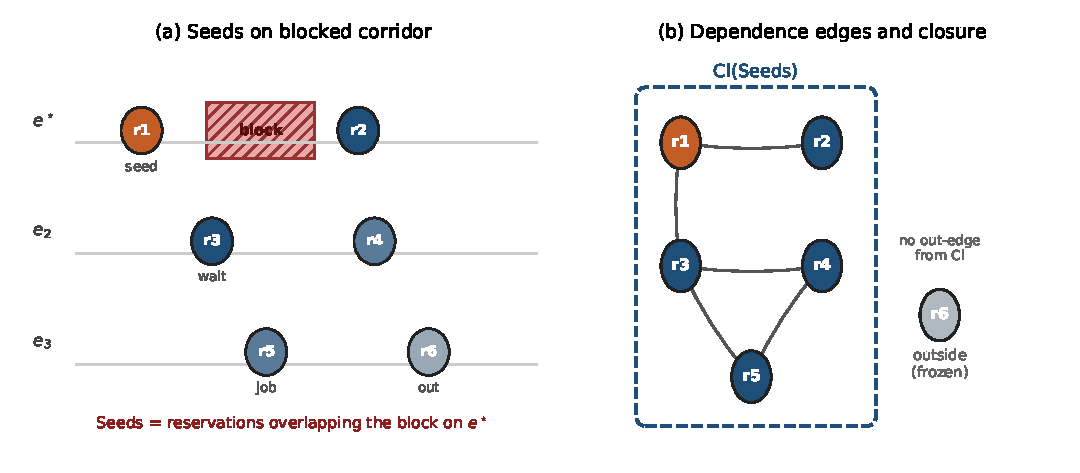
\includegraphics[width=\linewidth]{figures/fig_strc_closure}
\caption{时空预约闭包构造示意。
(a)~走廊阻断命中种子预约;
(b)~沿让行/接续边取传递闭包 \(\mathrm{Cl}(\mathrm{Seeds})\),外侧预约定向冻结。}
\label{fig:closure}
\end{figure}

对照的任务图边界臂(记 R1)将 \(T_{\mathrm{impact}}\) 映射为预约释放集:
凡任务标签属于影响域且 \(t^e>t_{\mathrm{now}}\) 的预约。
由命题~\ref{prop:miss},B 类上该集合为空;闭包臂(记 R2)取 \(U=\mathrm{Cl}(\mathrm{Seeds})\)。

\subsection{包含性}
\label{sec:containment}

\begin{prop}[结构闭合性]
\label{prop:struct}
对任意 \(S\subseteq R\),在 \(G_R^\circ\) 中不存在边
\(u\to v\) 满足 \(u\in\mathrm{Cl}(S)\) 且 \(v\in R^{\circ}\setminus\mathrm{Cl}(S)\)。
因而,从 \(\mathrm{Cl}(S)\) 出发沿出边无法到达闭包外的活预约。
\end{prop}

\begin{proof}
若存在这样的边 \(u\to v\),则由 \(u\in\mathrm{Cl}(S)\) 知存在活种子 \(s\) 使
\(s\to^* u\)。拼接 \(u\to v\) 得 \(s\to^* v\),故按定义~\ref{def:strc} 应有
\(v\in\mathrm{Cl}(S)\),矛盾。
\end{proof}

命题~\ref{prop:struct} 说明「局部」对应一个图论闭合对象:闭包外顶点不是任何
闭包内顶点的直接后继。它\emph{不}声称 \(G_R\) 已枚举物理世界中一切可能耦合——
边集是建模选择;一旦边集固定,闭合性就是定义的推论,而不是启发式半径。

\begin{prop}[外侧字段不变的充分条件]
\label{prop:outside}
设释放集 \(U=\mathrm{Cl}(S)\),并设第 1 级协调按第~\ref{sec:level1}~节执行:
(i)~禁行窗已写入路由层;(ii)~对每个 \(r\in R^{\circ}\setminus U\),将其原字段
\((e,[t^s,t^e),k)\) 预提交到新预约表且预提交成功;
(iii)~仅对 \(U\) 内运输调用路由器生成新占用;(iv)~最终排程通过无冲突校验。
则在恢复后的预约表 \(R'\) 中,每个外侧任务标签对应的占用字段与 \(\mathcal{S}^0\) 一致。
\end{prop}

\begin{proof}
由 (ii),外侧预约在重放开始前已按其原区间写入新表,且未与禁行窗冲突
(否则预提交失败)。步骤 (iii) 只为 \(U\) 内任务提交新占用,不删除或改写已提交的
外侧区间。因此,对外侧任务标签,新表中的 \((e,[t^s,t^e),k)\) 与预提交值相同,
亦即与 \(\mathcal{S}^0\) 相同。校验通过仅排除新占用与既有占用冲突,不改变已提交字段。
\end{proof}

\begin{remark}
若预提交因「外侧与禁行窗重叠」失败,则 \(S\) 未能覆盖全部直接命中预约,闭包种子不完备。
若协调因运输--工序衔接失败而触发第~\ref{sec:scope_escalation}~节扩域,则新的释放集
\(U'\supsetneq U\),命题~\ref{prop:outside} 只对最终未释放的外侧成立。
扩域以可行性优先于最小扰动,实验中单独报告。
\end{remark}

\subsection{结构可预测性}
\label{sec:structure}

在装卸点最小割更窄的布局上,同型 LU 割边阻断倾向于产生更大的相对闭包
(实验 E4)。该规律用于解释闭包规模的来源,统计稳定性有限时不作硬贡献。

%% =====================================================================
\section{闭包上的有界修复}
\label{sec:repair}
%% =====================================================================

图~\ref{fig:framework} 总览本文流程:先以 \STRC{} \emph{测量}释放集,
再在闭包上做第 1 级有界协调;失败则扩域重试。
对照臂 R1 仅替换释放集来源,R0+ 则打开热启动搜索——同一无冲突执行器上归因。

\begin{figure}[t]
\centering
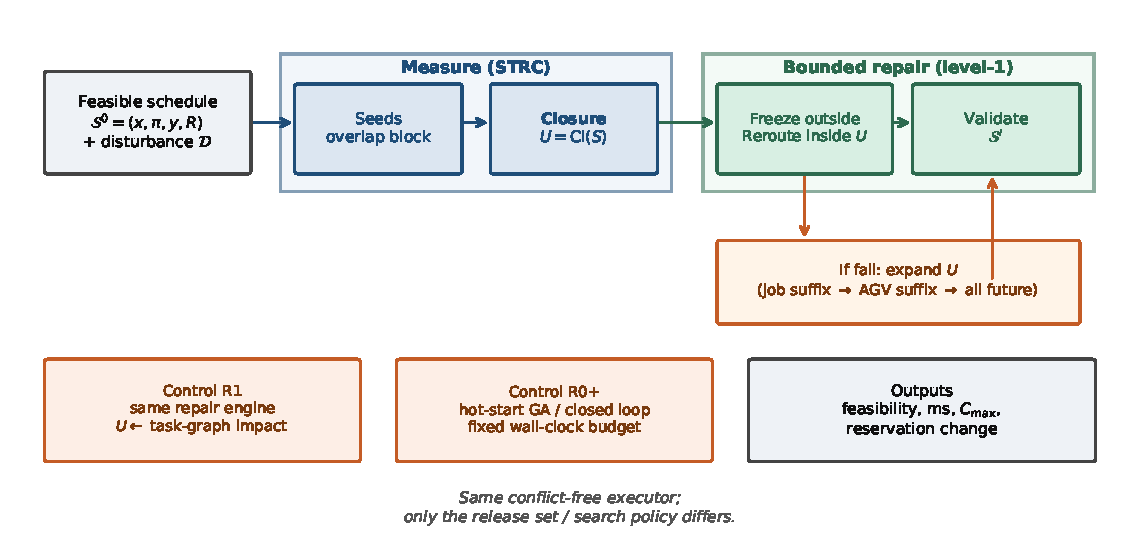
\includegraphics[width=\linewidth]{figures/fig_strc_framework}
\caption{\STRC{} 有界恢复框架。
上排:扰动下由种子取闭包并改路;中排:失败扩域;
下排:R1(任务图边界)与 R0+(热启动重解)对照及输出指标。}
\label{fig:framework}
\end{figure}

\subsection{释放、冻结与第 1 级改路}
\label{sec:level1}

给定释放集 \(U\),第 1 级协调保持原车辆指派与机器指派,按原扫描序重放:

\begin{enumerate}[leftmargin=1.4em,itemsep=0.2em]
\item 将扰动禁行窗写入路由层;
\item 对 \(r\notin U\) 的未来预约预提交到预约表(外侧冻结);若外侧已与禁行窗冲突,
    则闭包漏网,直接失败;
\item 对释放集内运输:原车在当前表上重规划空载/满载段并提交;
\item 推进机器空闲时刻与工件就绪时刻;以独立校验器验收,并禁止修复后占用仍落入禁行窗。
\end{enumerate}

该级不打开种群搜索。同引擎消融(E3)固定上述步骤,仅替换 \(U\) 来自 R1 或 R2,
用以把贡献归因于边界定义。

\subsection{失败扩域再修}
\label{sec:scope_escalation}

当外侧冻结过紧时,第 1 级可能因运输--工序衔接等校验失败。
此时不立刻求助于全局 GA,而按下列顺序扩大 \(U\) 并重试同一引擎:
(i)~并入释放集内各工序的同工件后缀未来预约;
(ii)~并入涉及车辆的同车后缀;
(iii)~必要时释放全部未来预约。
扩域仍是确定性单遍协调。扰动比例较小时,初始闭包偏紧、冻结偏多,扩域更常被触发;
比例较大时初始释放已较松,往往一轮成功。实验表明扩域可将可行率拉至全样本,
耗时仍保持在毫秒至十余毫秒量级(第~\ref{sec:experiments}~节)。

\subsection{与全局重解的对照}
\label{sec:vs_r0}

对照臂在相同禁行约束下,以 \(\mathcal{S}^0\) 的染色体热启动做固定挂钟预算的闭环搜索
(记 R0+)。它可改派与改序,因而更可能改善 \(C_{\max}\),但耗时由预算决定。
本文主张的角色分工是: \STRC{} 路径优先可行性与响应时间,
并在结构上限制释放集;R0+ 优先完工时间。
「外侧字段逐条不变」只在命题~\ref{prop:outside} 的条件下保证,实验中作部分观测。
交叉曲线与规模扫描用于展示互补,而非宣告单侧支配。

算法~\ref{alg:strc_repair} 与图~\ref{fig:framework} 对应:闭包界定 \(U\),
第 1 级改路,失败则按工件/车辆/全部未来依次扩域。

\begin{algorithm}[t]
\caption{基于 \STRC{} 的有界恢复(第 1 级 + 扩域)}
\label{alg:strc_repair}
\begin{algorithmic}[1]
\Require 排程 \(\mathcal{S}^0\), 扰动 \(\mathcal{D}\), 时刻 \(t_{\mathrm{now}}\)
\Ensure 排程 \(\mathcal{S}'\) 或失败
\State \(S \gets \mathrm{Seeds}(\mathcal{D})\);
      \(U \gets \mathrm{Cl}(S)\)
\For{轮次 \(=0,1,2,3\)}
  \State \(\mathcal{S}' \gets \textsc{ReplayReroute}(\mathcal{S}^0,\mathcal{D},U)\)
  \If{\(\mathcal{S}'\) 可行}
    \State \Return \(\mathcal{S}'\)
  \EndIf
  \State 按扩域规则更新 \(U\) \Comment{工件后缀 / 同车 / 全部未来}
\EndFor
\State \Return 失败
\end{algorithmic}
\end{algorithm}

%% =====================================================================
\section{实验}
\label{sec:experiments}
%% =====================================================================

\subsection{协议}
\label{sec:protocol}

\textbf{执行器与算例.}
下层路网、时间窗路由与独立校验器固定。扩样矩阵使用三算例
\(\texttt{example\_3x3x2}\)、\(\texttt{congested\_8x4x4}\)、
\(\texttt{S8x4x4}\)(high 布局)与种子
\(\{42,7,2024,99,123\}\)(共 \(15\) 个算例--种子对);
E4 另用 funnel/high 生成布局对。初始排程由冲突自由启发式解码得到。

\textbf{扰动.}
除非另注,\(t_{\mathrm{now}}=0.35\,C_{\max}(\mathcal{S}^0)\)。
E1--E3/E5 在繁忙走廊上施加单窗阻断;规模扫描将未来工序按最早未来预约排序,
取前比例 \(\varphi\) 的预约时窗作为微阻断(不合并)。

\textbf{对照臂.}
R1:任务图影响域 + 第 1 级改路;
R2/\STRC:闭包 + 第 1 级改路(规模扫描打开失败扩域;E3/E5 关闭扩域);
R0+:热启动闭环搜索,固定挂钟预算。

\subsection{E1:任务图漏报}
\label{sec:e1}

表~\ref{tab:e1} 与图~\ref{fig:e1e3}(左)汇总命题~\ref{prop:miss} 的扩样结果:
\(15/15\) 样本上 \(T_{\mathrm{impact}}=0\)、种子与闭包非空、阻断后原排程不可行,
结构泄漏均为 \(0\)。

\begin{table}[t]
\centering
\caption{E1 漏报(走廊阻断;每算例 \(5\) 种子)。均值取多种子平均。}
\label{tab:e1}
\small
\begin{tabular}{@{}lccccc@{}}
\toprule
算例 & \(n\) & C1 通过 & 均 \(|\mathrm{Seeds}|\) & 均 \(\mathrm{Cl}\) & 结构泄漏 \\
\midrule
\texttt{example\_3x3x2} & 5 & \(5/5\) & \(5.8\) & \(16.4\) & \(0\) \\
\texttt{congested\_8x4x4} & 5 & \(5/5\) & \(15.2\) & \(49.2\) & \(0\) \\
\texttt{S8x4x4} (high) & 5 & \(5/5\) & \(15.6\) & \(82.8\) & \(0\) \\
\bottomrule
\end{tabular}
\end{table}

\subsection{E2:包含性}
\label{sec:e2}

结构包含性(E2a)在 \(15/15\) 样本上成立(泄漏 \(=0\)),与命题~\ref{prop:struct} 一致。
第 1 级修复(无扩域)在 \(15/15\) 样本上可行。
外侧字段逐条不变(E2b / 命题~\ref{prop:outside} 的观测形式)在 \(7/15\) 样本上严格成立;
其余样本出现 \(1\)--\(5\) 条外侧字段漂移,表明当前依赖边集对部分弱耦合仍偏紧——
我们如实报告,并把加细边集列为后续工作,而不把 E2b 写成 \(100\%\)。

\subsection{E3:边界消融}
\label{sec:e3}

表~\ref{tab:e3} 与图~\ref{fig:e1e3}(右)固定第 1 级改路并\emph{关闭}失败扩域。
B 类上 \(15/15\) 样本 R1 释放集为空且不可行,R2 全部可行——贡献归因于边界定义。
若打开扩域,R1 可靠释放全部未来预约偶然可行,但已不再是任务图局部方法。

\begin{table}[t]
\centering
\caption{E3 边界消融(无扩域;三算例\(\times 5\)种子)。}
\label{tab:e3}
\small
\begin{tabular}{@{}lcccc@{}}
\toprule
算例 & miss\_B & R1 可行 & R2 可行 & R2 独胜 \\
\midrule
\texttt{example\_3x3x2} & \(5/5\) & \(0/5\) & \(5/5\) & \(5/5\) \\
\texttt{congested\_8x4x4} & \(5/5\) & \(0/5\) & \(5/5\) & \(5/5\) \\
\texttt{S8x4x4} (high) & \(5/5\) & \(0/5\) & \(5/5\) & \(5/5\) \\
\bottomrule
\end{tabular}
\end{table}

\begin{figure}[t]
\centering
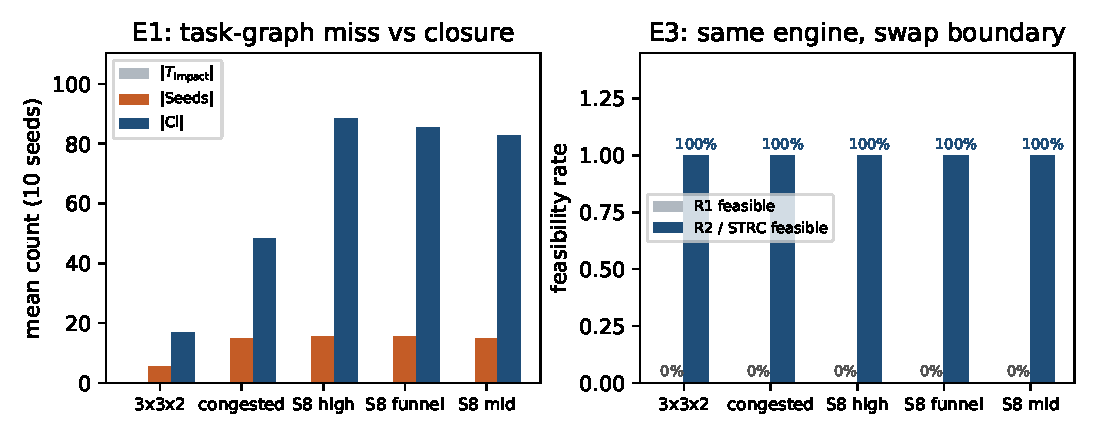
\includegraphics[width=\linewidth]{figures/fig_strc_e1e3}
\caption{E1/E3 扩样可视化(三算例\(\times 5\)种子均值)。
左:任务图影响域为空而种子与闭包非空;
右:同改路引擎下仅换边界时 R1 可行率为 \(0\)、R2 为 \(100\%\)。}
\label{fig:e1e3}
\end{figure}

\subsection{案例甘特}
\label{sec:case}

E1--E3 给出的是跨种子的计数与可行率。为把「任务图覆盖不到、闭包可修」落到时间轴上,
图~\ref{fig:case} 取 \(\texttt{example\_3x3x2}\)、种子 \(42\) 的一例走廊阻断
(与 E2/E3 同协议:\(t_{\mathrm{now}}=0.35\,C_{\max}\),繁忙走廊单窗阻断,第 1 级改路、无扩域)。

该例上 \(T_{\mathrm{impact}}=\varnothing\),而 \(|\mathrm{Seeds}|=6\)、\(|\mathrm{Cl}|=16\)。
图~\ref{fig:case}(a) 为扰动前原排程的机器甘特:蓝色工序的运输预约落入闭包(将被释放改路),
灰色工序在闭包外(预提交冻结);红色虚线为 \(t_{\mathrm{now}}\),浅红带为阻断时窗。
图~\ref{fig:case}(b) 为修复后:闭包内工序时间轴重排,排程在阻断下恢复可行,
\(C_{\max}:57\to 86\),耗时亚毫秒级。
本图不用于宣称完工时间最优——它只说明统计结论对应何种局部改动形态;
完工时间与全局重解的权衡见随后的 E5 与规模扫描。

\begin{figure}[t]
\centering
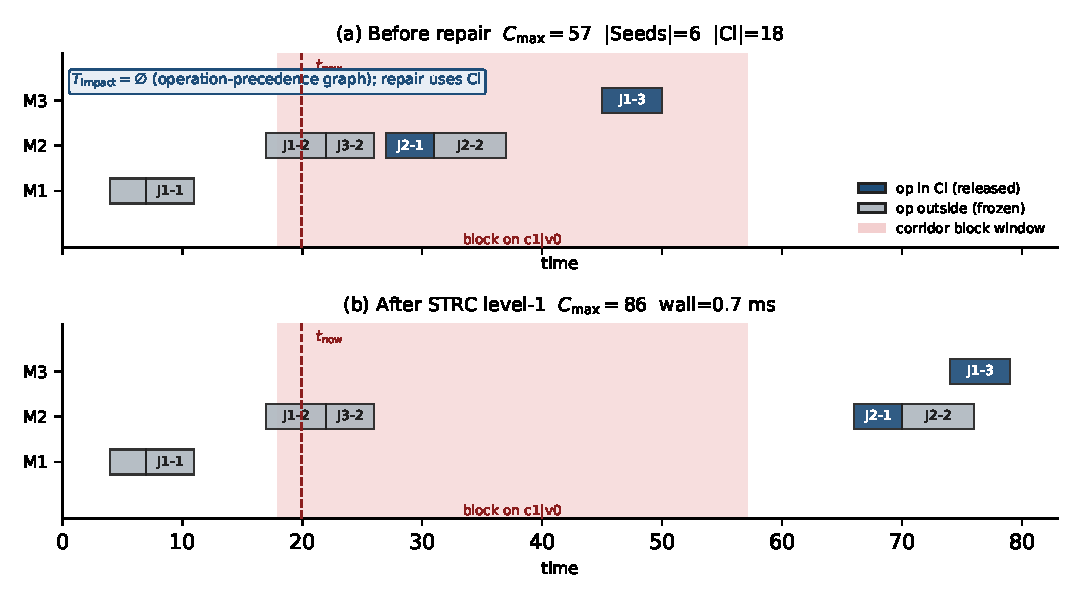
\includegraphics[width=\linewidth]{figures/fig_strc_case}
\caption{案例甘特(\texttt{example\_3x3x2}, seed \(42\))。
(a)~阻断前原排程,按是否属于 \(\mathrm{Cl}\) 着色;
(b)~STRC 第 1 级修复后。任务图影响域为空;蓝色工序对应闭包内运输被改路。}
\label{fig:case}
\end{figure}

\subsection{E4:结构(探索)}
\label{sec:e4}

在 LU 割边阻断下,funnel 与 high 的闭包占比随种子波动
(表~\ref{tab:e4});中位数上 funnel 高于 high,但均值不稳,故仅作结构解释。

\begin{table}[t]
\centering
\caption{E4 闭包占比 \(\mathrm{Cl}/|R|\)(LU 割边阻断;种子 \(42,7,2024,99,123\))。}
\label{tab:e4}
\small
\begin{tabular}{@{}lcccccc@{}}
\toprule
布局 & \(42\) & \(7\) & \(2024\) & \(99\) & \(123\) & 中位 \\
\midrule
funnel & \(0.254\) & \(0.181\) & \(0.296\) & \(0.309\) & \(0.180\) & \(0.254\) \\
high & \(0.156\) & \(0.204\) & \(0.372\) & \(0.229\) & \(0.184\) & \(0.204\) \\
\bottomrule
\end{tabular}
\end{table}

\subsection{E5:与全局重解的权衡}
\label{sec:e5}

图~\ref{fig:e5} 在 \(\texttt{congested\_8x4x4}\) 上对种子 \(\{42,7,2024\}\)
扫描 R0+ 预算 \(\{0.2,1,2\}\)\,s。
STRC(第 1 级,无扩域)均值约 \(1.8\)\,ms、\(C_{\max}\!\approx\!299\);
R0+ 随预算改善 \(C_{\max}\)(约 \(213\to 139\)),耗时高两至三个数量级。
互补性体现在速度/稳定性 vs 完工时间,而非第 1 级在 \(C_{\max}\) 上交叉反超。

\begin{figure}[t]
\centering
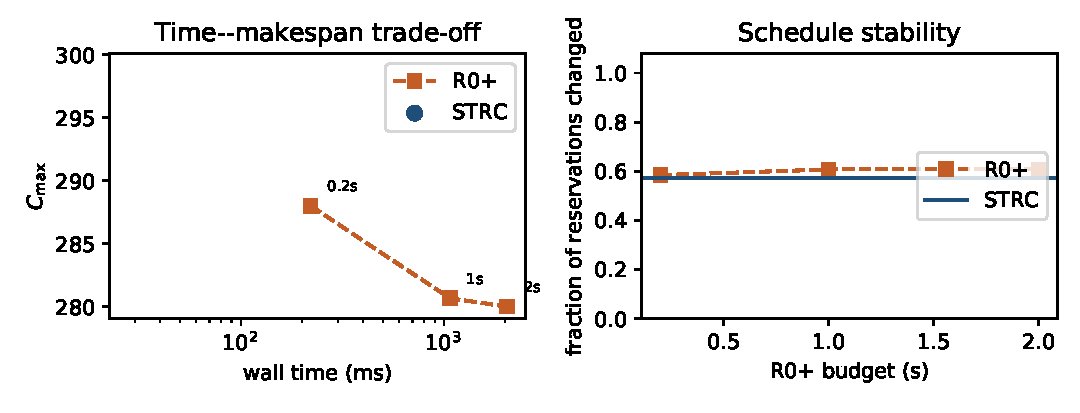
\includegraphics[width=\linewidth]{figures/fig_strc_e5}
\caption{E5:R0+ 预算扫描与 STRC 定点(\texttt{congested\_8x4x4}, \(3\) 种子均值)。
左:耗时--\(C_{\max}\);右:预约改动比例。}
\label{fig:e5}
\end{figure}

\subsection{扰动规模扫描}
\label{sec:scale}

表~\ref{tab:scale} 与图~\ref{fig:scale} 报告 \(\varphi\) 扫描
(\texttt{congested\_8x4x4}, \(5\) 种子; R0+ 预算 \(2\)\,s; STRC 含失败扩域)。
两臂可行率均为 \(100\%\); STRC 耗时约 \(4\)--\(9\)\,ms,R0+ 约 \(2\)\,s;
\(C_{\max}\) 均由 R0+ 更优。小例 \(\texttt{example\_3x3x2}\) 上同样 \(100\%\) 可行,
STRC 约 \(1\)\,ms 量级。

\begin{table}[t]
\centering
\caption{扰动规模对照(\texttt{congested\_8x4x4}, \(5\) 种子平均)。
STRC 含扩域;R0+ 预算 \(2\)\,s。}
\label{tab:scale}
\small
\begin{tabular}{@{}rccccc@{}}
\toprule
\(\varphi\) & STRC 可行 & STRC \(C_{\max}\) & STRC\,ms & R0+ \(C_{\max}\) & 耗时比 \\
\midrule
\(0.10\) & \(100\%\) & \(201\) & \(8.8\) & \(101\) & \(345\times\) \\
\(0.25\) & \(100\%\) & \(207\) & \(9.0\) & \(106\) & \(369\times\) \\
\(0.50\) & \(100\%\) & \(216\) & \(4.4\) & \(109\) & \(471\times\) \\
\(0.75\) & \(100\%\) & \(248\) & \(6.7\) & \(110\) & \(310\times\) \\
\(1.00\) & \(100\%\) & \(285\) & \(9.2\) & \(128\) & \(232\times\) \\
\bottomrule
\end{tabular}
\end{table}

\begin{figure}[t]
\centering
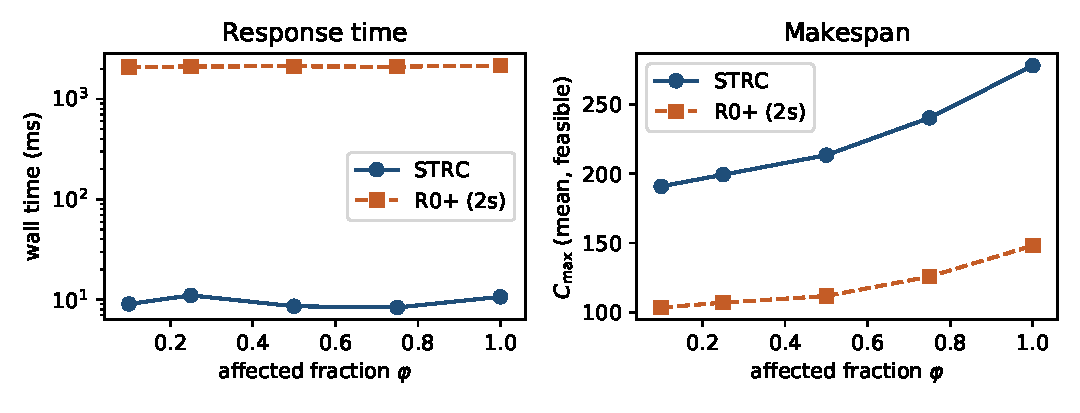
\includegraphics[width=\linewidth]{figures/fig_strc_scale}
\caption{扰动规模扫描(\texttt{congested\_8x4x4}, \(5\) 种子):
响应时间(对数轴)与完工时间随 \(\varphi\) 变化。}
\label{fig:scale}
\end{figure}

\subsection{小结}
\label{sec:exp_summary}

\begin{itemize}[leftmargin=1.5em,itemsep=0.25em]
\item 问题层(E1)与边界消融(E3)在 \(15\) 个算例--种子对上稳定成立;
案例甘特把同一协议落到工序时间轴。
\item 结构包含性(E2a)满通过;外侧字段严格不变(E2b)部分成立,边集仍可加细。
\item 与全局搜索互补(E5/规模扫描):毫秒级可行 vs 秒级更优 \(C_{\max}\)。
\item 不宣称第 1 级闭包修复在完工时间上全面优于全局搜索。
\end{itemize}


%% =====================================================================
\section{结论}
\label{sec:conclusion}
%% =====================================================================

本文指认了无冲突柔性作业车间中一类任务图覆盖不到的级联损坏,并将影响边界
重新定义在时空预约闭包(\STRC)上。在三算例\(\times 5\)种子的扩样上,
漏报与边界消融稳定成立;结构闭合性满通过,外侧字段逐条不变仅部分成立。
有界修复与失败扩域是闭包的应用。与热启动全局重解的对照支持
「测量与协调」和「搜索求质量」的角色分工。
局限与后续工作包括:加细预约依赖边集、A 类扰动上的系统对照、
升级阶梯中换车/改派级评估、多扰动并发,以及更强的结构可预测统计。

\bibliographystyle{ACM-Reference-Format}
\bibliography{reference-base}

\end{document}
